\documentclass[journal]{IEEEtran}
\hyphenation{op-tical net-works semi-conduc-tor}
\usepackage{cite}
\usepackage{times}
\usepackage{epsfig}
\usepackage{graphicx}
\usepackage{amsmath}
\usepackage{amssymb}
\usepackage{multirow}
\usepackage{booktabs}
\usepackage[table]{xcolor}
\usepackage{listings}
\usepackage{footnote}
\usepackage{bm}
\usepackage[normalem]{ulem}
\useunder{\uline}{\ul}{}
\usepackage{amsfonts} 
\usepackage{algorithm}
\usepackage{algorithmic}
\usepackage{times}
\usepackage{epsfig}
\usepackage{graphicx}
\usepackage{amsmath}
\usepackage{amssymb}
\usepackage{marvosym}

%%%%%%%%%%%%%%%%%%%%%%%%%%%%%%%%%%%%%%%%%%%%%%%%%%%%%%%%%%%%%%%%%%%%%%%%
%% 两种高亮标记：
%%  ① 黄底红字 \FILLIN{...}  = 还需作者填的空（本文件现已无，全部处理完）
%%  ② 青底 \AUTOVAL{...}     = Claude 从 Fig.\ref{ablavis} 图里 Otsu 估算的单图 IoU，
%%     数值现为作者在原图上粗算的 Full=0.79 / High=0.61 / Low=0.57（仍待与合作者复核确认）。
%%     确认无误后可把 \AUTOVAL{x} 直接改成 x（去掉青色高亮）。
%% 说明：F1 数据集名已按作者要求去掉（不点名具体数据集）；失败案例图 Fig.\ref{failurecase}
%%       已用 FANet 真实预测裁片，无需再填。
%%%%%%%%%%%%%%%%%%%%%%%%%%%%%%%%%%%%%%%%%%%%%%%%%%%%%%%%%%%%%%%%%%%%%%%%
\definecolor{fillorange}{RGB}{200,60,0}
\definecolor{fillyellow}{RGB}{255,242,0}
\newcommand{\FILLIN}[1]{\colorbox{fillyellow}{\textcolor{fillorange}{\textbf{[[TO FILL #1]]}}}}
% \AUTOVAL：青色高亮＝Claude 从图里估算的数值（作者需自行用模型复核后替换/确认）
\definecolor{autocyan}{RGB}{120,220,225}
\newcommand{\AUTOVAL}[1]{\colorbox{autocyan}{\textbf{#1}}}

\begin{document}

\title{Harnessing Frequency-Aware Network for 

Crack Detection in Road-Perceptive Autonomous Vehicles Scene}


\author{Senyun Kuang, Yintao Wei,

Yang Liu, and Xiaobo Qu,~\IEEEmembership{Senior Member,~IEEE}

\thanks{This work was supported by the National Natural Science Foundation of China [grant numbers 51761135124, 11672148, 52003142, 51775293]; and the State Key Laboratory of Vehicle NVH and Safety echnology [Grant number NVHSKI-202106]. The authors are with the State Key Laboratory of Automotive Safety and Energy, Tsinghua University, Beijing 100084, China. The emails of these authors are: ksy23@mails.tsinghua.edu.cn, weiyt@tsinghua.edu.cn, xiaobo@tsinghua.edu.cn and liuy@chalmers.se.}}

\markboth{Submit to IEEE Transactions on Cybernetics}%
{Shell \MakeLowercase{\textit{et al.}}: Bare Demo of IEEEtran.cls for IEEE Journals}

\maketitle


\begin{abstract}
With the evolution of intelligent transportation systems, the integration of crack detection capabilities in vehicles has seen significant advancements. Existing deep-learning based crack detection methods, predominantly focused on the RGB domain, often fall short in complex scenarios where cracks blend seamlessly with their background. Recognizing that road cracks and surrounding pavement features exhibit greater discriminative potential in the frequency domain, we introduce a novel frequency-aware mechanism. Our frequency-aware network (FANet), operates in two step: a frequency-guided coarse crack localization step for initial crack identification, followed by a detail-preserving fine crack segmentation for enhanced precision. Leveraging different features from the backbone, FANet employs frequency-aware module for effective coarse positioning. Subsequently, a hybrid fusion module meticulously integrates high-level features via prior-guided corrections, further refining detection by incorporating shallow features for detailed correction of detected cracks. Empirical evaluations on five datasets demonstrate FANet's superior performance.
\end{abstract}

\begin{IEEEkeywords}
Crack Detection, Frequency-aware Feature Learning, Road-perceptive Vehicles
\end{IEEEkeywords}


\section{Introduction}\label{sec1}

Maintaining the structural integrity of infrastructure is paramount, with crack detection playing a crucial role in safeguarding facilities against the detrimental effects of deterioration. Timely detection and remediation of cracks are essential for preventing potentially irreversible damage. The advent of autonomous vehicles and advanced environmental perception technologies~\cite{DBLP:journals/tcyb/HuzaefaL23,DBLP:journals/tcyb/CaoRS23,DBLP:journals/tcyb/ZhangLLGGCL24} heralds a new era in automated road condition monitoring, with autonomous road-perceptive vehicles poised to revolutionize how we maintain our roadways~\cite{9543474,
mohan2018crack,9998084,
DBLP:journals/tcyb/XieWLLLWZJ24,Almaskati2024}. Integrating crack detection capabilities into these vehicles offers a promising pathway for continuous road condition surveillance~\cite{Zhang2024}.

\begin{figure}
\centering

\includegraphics[width=0.83\linewidth]{IEEEtran/spider0330.pdf}
\caption{{Performance of our proposed method and other methods, including AFFMM~\cite{DBLP:journals/tits/QuCWYL22} and MSFE~\cite{DBLP:journals/tiv/ZhouQJ23}, in Crack500~\cite{DBLP:journals/tits/YangZYPML20}, GAPs384~\cite{DBLP:conf/ijcnn/EisenbachSSADSE17}, CrackTree200~\cite{DBLP:journals/prl/ZouCLMW12}, CFD~\cite{DBLP:journals/tits/ShiCQMC16} and AEL~\cite{DBLP:journals/tits/AmhazCIB16}.}}
\label{introdvis}
\end{figure}

\begin{figure*}[!t]
\centering

\includegraphics[width=0.95\linewidth]{IEEEtran/car0331.pdf}
\caption{The road-perceptive vehicle may contain three steps. The first is to take photos of road condition. The second is to detection the crack by our proposed method. The third is to analysis the result and send back to vehicles.}
\label{road-perceptive vehicle}
\end{figure*}


Traditional crack detection methods have primarily relied on digital image processing technologies, involving laborious procedures with complex preprocessing and initial crack identification, followed by refinement~\cite{DBLP:conf/icarcv/DinhHL16,DBLP:journals/tits/OliveiraC13}. These techniques, dependent on manually selected features and classical machine learning models, often falter when distinguishing cracks against intricate backgrounds. The advent of deep learning marks a pivotal transition, ushering in a wave of sophisticated algorithms designed for specific types of cracks and conditions. This shift leverages the capabilities of convolutional neural networks (CNNs) to significantly improve road damage detection, utilizing hierarchical feature learning for edge detection~\cite{DBLP:journals/ijon/LiuYLXL19,DBLP:journals/tits/YangZYPML20} and pioneering deep supervision and enhancement techniques for heightened performance. Moreover, multi-scale feature fusion has emerged to effectively marry local and global feature representations, with attention mechanisms fine-tuning feature selection for better discrimination~\cite{DBLP:journals/wicomm/HuHYHL21,DBLP:journals/cacie/QuqaLL23,li2018automatic}.

Despite these advancements, deep learning methods predominantly focus on the RGB domain, searching for textural inconsistencies or `breakthrough points' to pinpoint cracks. Yet, the nuanced characteristics of road surfaces frequently mask these defects, posing significant detection challenges. 


%%%%%%%%%%%%%%%%%%%%%%  R1 - Q1 %%%%%%%%%%%%%%%%%%%%%%



Recently, several studies have introduced frequency-domain cues into image segmentation, such as FsaNet~\cite{DBLP:journals/tip/ZhangPG23}, LGFFM~\cite{11129883TMI}, FMamba~\cite{DBLP:journals/tim/LiuLLWZS25}, and FINet~\cite{DBLP:journals/tcsv/WangZZGY25}. 
Although these methods validate the potential of frequency features, they typically treat frequency information as auxiliary input rather than achieving a deeply coupled frequency-spatial representation. 
For instance, FsaNet focuses only on low-frequency tokens without adaptive fusion with spatial branches, LGFFM employs dual encoders with heavy computation, FMamba emphasizes global consistency while losing fine texture detail, and FINet is restricted to ultrasound imagery. 
These limitations reveal that existing frequency-based networks lack generalization and efficient integration with spatial representations, especially in complex natural scenes.


%%%%%

Addressing this, our study introduces the Frequency-aware network (FANet), a novel architecture that integrates RGB and frequency domain information. This dual-strategy approach aims to overcome the limitations of relying solely on RGB information by enhancing the network's sensitivity to subtle textural features often obscured in the spatial domain. FANet represents a significant leap forward, offering enhanced accuracy in crack detection through a more holistic analysis of road surface characteristics.
FANet commences its detection process with a frequency-guided coarse positioning phase, where the primary aim is to leverage frequency domain features for identifying potential crack locations, known as breakthrough points. Distinguished by a transformer backbone, FANet proficiently extracts different level features from the input. A specialized frequency-aware module (FAM) then distinguishes these features into high- and low-frequency components, which correspond to the texture and contour details of the road surface, respectively. This division allows for a comprehensive representation of the frequency domain, enabling the coarse but accurate localization of road cracks. The process is enhanced by a neighbor interaction mechanism that promotes the integration of frequency-aware features across various levels, facilitating an initial yet refined crack detection.

Transitioning into the detail-preserving fine segmentation phase, FANet refines the previously identified crack locations through a process of prior-guided correction and cross-layer feature fusion. This refinement is achieved with the help of the hybrid fusion module (HFM), which manages the interplay of high-level features across different layers to boost the accuracy of the detection framework. The inclusion of shallow, high-resolution features ensures the meticulous delineation of structural information, leading to the production of the final crack detection output. This dual-phase approach, combining coarse positioning with fine localization, allows FANet to not only detect cracks with high precision but also to discern subtle features that traditional methods might overlook, setting a new standard in the field of road surface monitoring. In Fig. \ref{introdvis}, our proposed framework demonstrates superior performance across all five datasets. 

The core contributions of this paper are listed as follows:

\begin{itemize}
    
    
    \item We propose a two-stage Frequency-Aware Network (FANet) that jointly models spatial and frequency information for robust crack detection. 
    Unlike existing approaches that process frequency cues independently, FANet achieves unified frequency-spatial representation through frequency-guided coarse localization and detail-preserving fine segmentation, 
    significantly enhancing precision and generalization under complex textures and noise.

    \item We design a fully integrated frequency-aware module capable of automatically distinguishing between low- and high-frequency features. This module significantly improve the the localization of road cracks.
    
    \item We introduce a hybrid fusion module meticulously integrates high-level features via prior-guided corrections, further refining detection by incorporating shallow features for detailed correction of detected cracks. The performance in five different datasets demonstrates the effectiveness of our FANet.
    
\end{itemize}


\section{Related Work}\label{sec2}


\subsection{Traditional Crack Detection Techniques}
For traditional crack detection, Techniques such as intensity thresholding, morphological analysis, and classical machine learning strategies have been foundational, as evidenced by extensive different researchs~\cite{DBLP:journals/cacie/NishikawaYSF12,DBLP:journals/cacie/YangLYLHY18}. A pioneering approach within this domain is the CrackTree algorithm, delineated in~\cite{DBLP:journals/prl/ZouCLMW12}, which utilizes minimum spanning trees (MSTs) for the automated identification of cracks. Parallel to this, substantial efforts by researchers~\cite{DBLP:journals/ivc/LiZZM11,DBLP:journals/pami/KaulYT12,DBLP:journals/tits/AmhazCIB16} have been devoted to leveraging minimal path techniques for crack region detection. Given the complex, irregular patterns of cracks, numerous strategies have been formulated, emphasizing edge detection and bespoke feature engineering. An innovative methodology reported in~\cite{DBLP:journals/ivc/ZhangLCCHZ17} implements a dual-phase strategy, initiating with Region of Belief (RoB) seed extraction, succeeded by region-growing algorithms to coalesce disjointed regions for enhanced crack identification. Furthermore, the technique introduced in~\cite{DBLP:journals/tits/ShiCQMC16} makes use of random structure forests in crack detection, thereby facilitating a better comprehension of crack structures and diminishing noise artifacts. Nonetheless, these traditional methods, despite their utility in specific contexts, are often challenged by their susceptibility to noise and a heavy reliance on manual feature extraction, limiting their effectiveness in more intricate scenarios.



\begin{figure*}[!hbpt]
\centering

\includegraphics[width=\linewidth]{IEEEtran/framework1019.pdf}
\caption{Overall architecture of the proposed Frequency-Aware Network (FANet). 
The solid arrows denote feature flow between modules, while dashed lines represent skip connections used for cross-layer feature fusion. 
Each block (FAM, HFM, and Transformer-based backbone) corresponds to a specific processing stage described in Sections~\ref{overview} to~\ref{sec:Detail-preserving-Fine-Localization}.}
\label{Framework}
\vspace{-0.5cm}
\end{figure*}




\subsection{Advancements in Crack Detection via Deep Learning}

The realm of crack detection has witnessed a transformative shift with the advent of deep learning technologies, heralding a new epoch of innovation and efficiency. This period is characterized by breakthroughs in deep learning that have revolutionized not only detection but also classification and segmentation within various fields~\cite{Hu2025,DBLP:journals/pami/ChenLLSWZ21,KUANG2024100146,PENG2025100170}. Central to these advancements is the ability of deep learning models to autonomously discern and abstract pivotal, high-level features via an end-to-end learning process. 
This capability has driven rapid progress in applying deep learning to crack detection tasks~\cite{DBLP:journals/cacie/RodriguezLozanoGPO23, DBLP:journals/cacie/ZhouZG23}.



For example, an innovative hierarchical segmentation network that integrates FCNs with Conditional Random Fields (CRFs) and Guided Filtering (GF) is introduced in~\cite{DBLP:journals/ijon/LiuYLXL19}, aiming to exploit multi-layer features for meticulous refinement. Following this, encoder-decoder based FCNs have been developed, tailored to discriminate between crack and non-crack pixels with high precision~\cite{DBLP:journals/LD}. The DeepCrackT model, as proposed in~\cite{DBLP:journals/tip/ZouZLQWW19}, enhances the encoder-decoder framework through a novel pairwise fusion technique of crack features at corresponding scales, significantly boosting detection capabilities. In pursuit of computational efficiency, the introduction of a lightweight crack detection network marks a significant milestone, incorporating split-exchange convolution and multi-scale feature fusion to streamline network operations and expedite detection processes~\cite{DBLP:journals/tiv/ZhouQJ23}.

However, relying solely on RGB information presents a significant limitation~\cite{ZHUANG2025100194}, as the spatial domain represented by RGB channels provides a direct yet occasionally superficial perspective of image content, potentially overlooking subtle features more discernible in the frequency domain. Recognizing this shortfall, our work introduces an innovative approach that incorporates frequency domain information into the crack detection process. By leveraging the frequency domain, we aim to reveal a wider spectrum of features, leading to more accurate and robust crack detection.


In addition to conventional RGB-based frameworks, several recent studies have explored incorporating frequency-domain cues into image segmentation. 
For instance, FsaNet~\cite{DBLP:journals/tip/ZhangPG23} applies a discrete cosine transform (DCT) to enhance low-frequency representations, 
yet it lacks adaptive interaction between frequency and spatial branches, limiting its generalization to texture-rich or noisy environments. 
LGFFM~\cite{11129883TMI} introduces a dual-encoder structure combining CNN and Transformer backbones along with a Frequency Domain Mapping Module, 
which improves global perception but incurs high computational complexity and training instability. 
FMamba~\cite{DBLP:journals/tim/LiuLLWZS25} embeds frequency enhancement into a lightweight Vision Mamba backbone, 
providing efficient feature extraction but prioritizing sequential consistency rather than fine-grained local texture cues. 
FINet~\cite{DBLP:journals/tcsv/WangZZGY25} proposes a frequency-aware self-attention mechanism for ultrasound image segmentation, 
but it is task-specific and not easily generalizable to natural road scenes.




These methods collectively demonstrate the potential of frequency features in segmentation, 
yet they generally treat frequency cues as auxiliary enhancements rather than deeply integrating them with spatial representations. 
\textbf{In contrast, our proposed FANet establishes a unified two-stage frequency-spatial synergy, 
where the frequency-guided coarse localization phase captures global structure and the detail-preserving fine segmentation phase refines local details.} 
This design enables dynamic modulation between spectral and spatial features, achieving superior robustness, precision, and adaptability under complex road textures and illumination variations.

\textcolor{red}{More recent studies from the past two years further advance both crack detection and frequency-aware representation learning. On the crack-detection side, UP-CrackNet~\cite{TITS24_UPCrackNet} formulates road crack detection as unsupervised adversarial image restoration to remove the dependence on pixel-wise annotations; SCSegamba~\cite{CVPR25_SCSegamba} designs a lightweight structure-aware vision Mamba that captures crack morphology and texture with minimal computational cost; and an ultra-lightweight Mamba network with frequency-domain feature extraction has been developed for pavement tiny-crack segmentation~\cite{ESWA25_MambaFreqCrack}. On the frequency-modeling side, FreqFusion~\cite{TPAMI24_FreqFusion} rectifies feature fusion for dense prediction with adaptive low-/high-pass filters, and FSEL~\cite{ECCV24_FSEL} entangles frequency and spatial representations for camouflaged object detection. Closely related inspection and segmentation problems have also been actively studied in IEEE Transactions on Cybernetics, including zero-shot industrial anomaly detection with hybrid vision-language prompts~\cite{TCYB25_AnomalyVLM} and contrastive transformer-based segmentation of subtle structures~\cite{TCYB24_CTNet}. These advances confirm the growing interest in spectral cues and efficient architectures; however, they either address generic dense prediction or treat frequency information as an auxiliary enhancement, leaving a deeply coupled frequency-spatial representation dedicated to road crack detection, the very focus of FANet, largely unexplored.}





\section{Proposed Method}
\subsection{Overview} \label{overview}
Our objective is to harness and integrate the unique benefits of both the RGB and frequency domains, aiming to boost the discriminative capabilities for detecting road cracks via intelligent road-perceptive vehicles. In pursuit of this, we present the FANet, a novel architecture tailor-made for crack detection, as depicted in Fig.~\ref{Framework}. FANet is architected around three core components: the Transformer-based feature extraction, the frequency-guided coarse crack localization step, and the detail-preserving fine crack segmentation step. Given an input image $S \in \mathbb{R}^{H \times W \times 3}$, FANet begins with the feature extraction with the Pyramid Vision Transformer (PVT)~\cite{DBLP:journals/cvm/WangXLFSLLLS22} as its feature extractor. This feature extractor generates multi-level feature maps $F_i$, $i \in \{1,2,3,4\}$, each catering to different facets of the detection challenge. The first-level feature map $F_1$, captures intricate details of the road surface essential for spotting minor cracks, whereas the subsequent levels ($F_2, F_3, F_4$) encapsulate progressively higher-level semantic information, pivotal for robust crack localization. In the frequency-guided coarse crack localization phase, our proposed novel frequency-aware module (FAM) extracts frequency domain features from the high-level features ($F_2, F_3, F_4$), which are then synergized using a {tri-merge (T-M) decoder}. This process yields a preliminary crack map $S_1$. 

After the coarse step, the detail-preserving fine crack segmentation step refines the initial map by using $S_1$ to steer the embedding of high-level features into a hybrid fusion module (HFM). This module facilitates layer-wise, prior-guided adjustments and fusion, significantly enhancing segmentation accuracy. After this step, the final ouput crack map is $S_{\text{output}}$.

\begin{figure}
\centering

\includegraphics[width=0.75\linewidth]{IEEEtran/HFM_0617.pdf}
\caption{{The architecture of our proposed hybrid fusion module (HFM).}}
\label{HFM}
\vspace{-0.5cm}
\end{figure}

\subsection{{Frequency-guided Crack Localization}} \label{sec:Frequency-guided-Coarse-Positioning}
Leveraging the concept that predators' hunting mechanisms often rely on frequency information to detect subtle anomalies in natural environments, we posit that similar advantages can be applied to road crack detection. This hypothesis is grounded in observations that frequency domain methods, traditionally used in camouflaged object detection, can significantly enhance the detection of subtle road anomalies. Conventional techniques typically employ the DCT to transition from RGB to the frequency domain, a process that, despite its effectiveness, is hindered by the lack of flexibility due to offline processing requirements. However, recent advancements like the work~\cite{DBLP:conf/iccv/Chen0XYKRYF19} have introduced the use of octave convolutions, which enable the partitioning of image data into high and low-frequency components directly, thereby streamlining the detection workflow. 



\textcolor{red}{\textbf{Design intuition of FAM.} Road cracks appear as sparse and sharp intensity discontinuities embedded in slowly varying pavement context. In the feature space, the former concentrates in the high-frequency band, whereas the latter dominates the low-frequency band. The FAM is therefore designed to (i) decompose each backbone feature into a high-frequency and a low-frequency component, (ii) let the two components exchange complementary information, so that edge responses acquire contextual support and contour responses are cleansed of texture noise, and (iii) adaptively re-weight and merge the two bands with learnable gates. The output is a frequency-balanced feature in which crack evidence is amplified relative to the background texture. The remainder of this subsection formalizes these three steps.}

In Octave Convolution~\cite{DBLP:conf/iccv/Chen0XYKRYF19},
feature maps are explicitly factorized into high- and low-frequency components along the channel dimension,
represented as $\{F_i^h, F_i^l\}$. 
The high-frequency branch $F_i^h$ captures rapidly varying fine-grained textures and edges, 
while the low-frequency branch $F_i^l$ models smoothly varying contextual structures by operating at a lower spatial resolution (typically half). 
This separation enables the network to process detailed and structural information in a complementary way, 
providing an efficient approximation of frequency decomposition within the spatial domain.




These low-frequency components often represent smooth regions, such as uniform road surfaces, whereas high-frequency elements are indicative of potential cracks or damage due to their significant intensity variations. Inspired by the work~\cite{DBLP:conf/iccv/Chen0XYKRYF19}, we explicitly factorize $F_i$ and get the high- and low-frequency components $\{F_i^h,F_i^l\}$.

Our proposed FAM achieves dynamic, end-to-end frequency information processing, facilitating the direct learning of crack characteristics in real-time. This approach not only avoids the limitations associated with DCT but also benefits from the computational prowess of GPUs, allowing for efficient integration into diverse network structures. As shown in Fig. \ref{Framework}, the FAM process $f^*_{i} = \{f^{h}_{i},f^{l}_{i}\}$ is mathematically represented as follows:

\begin{equation}
f^{h}_{i} = Conv(F^{h}_{i}) + \text{Upsample}(Conv(F^{l}_{i}), 2),
\end{equation}

\begin{equation}
f^{l}_{i} = Conv(F^{l}_{i}) + Conv(\text{Pool}(F^{h}_{i}, 2)),
\end{equation}
where $\text{Pool}(X, k)$ represents average pooling with a $k \times k$ kernel, and $\text{Upsample}(X, s)$ signifies upsampling by a scale factor of $s$ through nearest neighbor interpolation. 

Considering the significance of both high-frequency texture attributes for detailing surface irregularities and low-frequency contour attributes for outlining the broader features of the road surface, we integrate these components to form a comprehensive representation of frequency domain information tailored for road crack detection:
\begin{equation}
f_i = \{ \text{Resize}(f^{h}_{i}) \odot W^{h}_{i} \} \oplus  \{ \text{Resize}(f^{l}_{i})  \odot W^{l}_{i}  
 \},
\end{equation}
where $\text{Resize}$ denotes the operation to adjust features to a uniform dimension, $W^{h}_{i}$ and $W^{l}_{i}$ are learnable parameters, and $\oplus$ represents the element-wise addition. 
Here, $\odot$ denotes the element-wise multiplication.


\textcolor{red}{\textbf{Design intuition of T-M.} The T-M decoder aggregates the frequency-aware features of the three deepest levels: deeper features indicate \emph{where} a crack is likely to exist, while shallower ones describe its shape more precisely. Multiplying adjacent levels retains only the responses that are confirmed by both, yielding a clean coarse localization map $S_1$.}

The purpose of the frequency-guided coarse crack localization step is to initially locate the crack position. In order to fully utilize the effectiveness of the different features, we designed the T-M decoder so as to predict the crack location. This decoder leverages the semantic richness across layers via connections between adjacent layers, fostering a comprehensive feature representation as:

\begin{equation}
\begin{split}
    f'_3 &= Conv^ {\uparrow }(f_4)   \odot f_3, \\
    f'_2 &= Conv^ {\uparrow }(f_3)   \odot f_2, \\
    f'_{t-m} &= \text{Cat}(f_2,f'_2)  \odot \text{Cat}(f_2,f'_3).
\end{split}
\end{equation}

Herein,  $Conv^ {\uparrow }$ represents upsampling followed by a $3 \times 3$ convolution, 
and $\text{cat}(A, B)$ denotes the concatenation of features $A$ and $B$. 
The culmination of this phase is $f'_{t-m}$, leading to the formation of a coarse crack detection map $S_1$, 
signifying the initial phase of road crack identification.



\subsection{{Detail-preserving Crack Segmentation}} \label{sec:Detail-preserving-Fine-Localization}

Upon the coarse localization via frequency-domain insights, we underscore the importance of refining these detections to ensure both completeness and precision. To this end, we introduce a detail-preserving segmentation strategy, crucial for the nuanced delineation of crack structural information. This approach enhances the integration of high-level features with prior corrections and channel associations, alongside the utilization of high-resolution features for accurate structural information mapping, as depicted in Fig.~\ref{Framework}.

Central to this strategy is the HFM, shown in Fig. \ref{HFM}, a construct designed to seamlessly integrate features across layers, enriched by the insights from a coarse crack detection map $S_g = \{S_1, S_2\}$. To boost computational efficiency while retaining detection fidelity, input feature channels are initially condensed to 64, symbolized as $F_i$ and $F_{i+1}$.

\textcolor{red}{\textbf{Design intuition of HFM.} The HFM addresses two questions during refinement. The first is \emph{where to refine}: the coarse map $S_g$ acts as a spatial prior that amplifies crack-relevant regions of the deeper feature. The second is \emph{what to keep}: a channel-level association between adjacent layers determines which high-resolution details are consistent with this prior and should be preserved. Both operations are lightweight, so the refinement improves accuracy at a marginal computational cost. The following formulation details the two steps.}

%3-6
The HFM leverages the coarse crack detection map $S_g$ as a spatial prior to refine subsequent layer features by modulating their activation intensity in crack-relevant regions. 
Specifically, $S_g$ is multiplied with the feature maps $F_{i+1}$ to generate a prior-weighted response that emphasizes potential crack areas while suppressing irrelevant background noise. 
This guided interaction enables the network to iteratively refine feature representations, achieving more accurate and stable crack localization across layers.
This process is articulated through the multiplication of $F_{i+1}$ with $S_g$, followed by upsampling to achieve refined feature outputs $f^r_{i+1}$:


%%%%

\begin{equation}
f^r_{i+1} = \text{Upsample}(F_{i+1} \otimes S_g).
\end{equation}

Given the richness of channel-specific cues in high-level features, the key to augmenting cross-layer feature dialogue and the module engages in channel-level association. This mechanism evaluates pixel-wise similarity across channels, employing a $3 \times 3$ convolution to construct a bottleneck, thus optimizing output channel dimensions:

\begin{equation}
A = Conv(F_{i} \odot (f^r_{i+1})).
\end{equation}

Subsequent steps involve deriving two weight maps, $\alpha$ and $\beta$, from the feature matrix $A$ via dual $3 \times 3$ convolutions. These weights dynamically modulate $F_{i}$ features, facilitating an advanced synthesis of cross-layer information:

\begin{equation}
f^{out}_{i} = f^r_{i+1} + Conv(F_{i}) \times \alpha + \beta.
\end{equation}


To complement these advanced techniques with detailed spatial insights, 
we use two $3 \times 3$ convolutions to generate the final output $S_{\text{output}}$.

%%%%%%%%%%%%%

\textbf{Loss Function.} In alignment with standard practices, we train the FANet through binary cross-entropy loss:
\begin{equation}
L = BCE(S_{\text{output}},\mathcal{G}^T),
\end{equation}
where $\mathcal{G}^T$ is the ground-truth.


%%%%%%%%%%%%%%%%%%%%%%%%%%%%%%%%%%%%%%%%%%%


\begin{figure*}[!t]
\centering

\includegraphics[width=0.9\linewidth]{IEEEtran/com0322.pdf}
\caption{Comparison between our FANet and other SOTA methods. It can be clearly observed that FANet achieves impressive performance in all these cases. Best viewed by zooming in.}
\label{QualitativeResults}
\end{figure*}


\section{Experiments}
\subsection{Implementation Details}
FANet builds on the PVT in PyTorch pre-trained on ImageNet. We use the Adam optimizer, starting with a learning rate and weight decay of $1e-4$. Input image are resized to $512 \times 512$, and we train for 100 epochs on an NVIDIA 3090Ti GPU, with mini-batches of 4. Data augmentation strategies like random flipping and cropping are employed to improve robustness.





\subsection{Datasets for Evaluation}
Our model's efficacy is rigorously assessed using five widely recognized datasets, each offering unique challenges that simulate the complexities of crack detection scenarios.

\textbf{Crack500}~\cite{DBLP:journals/tits/YangZYPML20}: A comprehensive dataset tailored for crack detection, Crack500 consists of 500 images, partitioned into 250 for training, 50 for validation, and 200 for testing. It encompasses a diverse array of crack conditions, including but not limited to occlusions, variable contrast, shadow effects, and ambient noise, accurately mirroring the intricate nature of real-life crack detection challenges.

\textbf{GAPs384}~\cite{DBLP:conf/ijcnn/EisenbachSSADSE17}: Designed to tackle the intricacies of extreme lighting conditions on road surfaces, GAPs384 categorizes cracks into two distinct categories based on lighting: excessively dark and overly bright areas. This categorization underlines the challenge of distinguishing between cracks under varying lighting conditions. The dataset is comprised of 384 images, meticulously annotated to facilitate detailed analysis, with image dimensions of either $640 \times 540$ or $440 \times 540$.

\textbf{CFD}~\cite{DBLP:journals/tits/ShiCQMC16}: Specializing in cracks on concrete surfaces, the CFD dataset includes 118 images, each sized at $480 \times 320$. The dataset is characterized by its portrayal of common real-world disturbances such as uneven lighting, shadows, obstructions, and moisture accumulation, thus providing a robust platform for evaluating crack detection algorithms.

\textbf{Cracktree200}~\cite{DBLP:journals/prl/ZouCLMW12}: Comprising 206 images of pavement cracks at a resolution of $800 \times 600$, Cracktree200 emphasizes the detection of slender crack formations. The dataset is notable for its representation of fine cracks amidst complex backgrounds, including tree shadows, ambiguous road markings, and the intersection of cracks with such road features.



\textbf{AEL}~\cite{DBLP:journals/tits/AmhazCIB16}: The AEL dataset amalgamates three subsets: Aigle-RN, ESAR, and LCMS. Aigle-RN includes 38 pixel-annotated images for the assessment of French pavements, whereas ESAR and LCMS offer 15 and 5 images, respectively, without specified lighting conditions, further diversifying the dataset's utility in crack detection research.



%%%%%%%%%%%%%%%%%%%%




%%%%%%%%%%%%%%%%%%%%%%%%%%%%%%%%%%%%%%%%%%%


%%%%%%%%%%%%%%%%%%%%%%%%%



%%%%%%%%%%%%%%%%%%%%%%%%%%%%   3  %%%%%%%%%%%%%%%%%%%%%%%%%%%%%%



%%%%%%%%%%%%%%%%%%%%



\begin{table*}[]
\centering
\caption{{Comparison of our proposed method's performance with other methods using F1, AIU, and AP metrics across five datasets. 
Higher values in F1, AIU, and AP indicate superior performance. 
Values highlighted in \textcolor{red}{red} indicate the best performance, while values in \textcolor{green!50!black}{green} represent the second-best results for each dataset.}}
\scalebox{0.7}{
\begin{tabular}{@{}cc|cccccccccccccccccc@{}}
\toprule
\multicolumn{2}{c|}{}                                           & \multicolumn{18}{c}{Method}                                                                                                                                                                                                                                                                                                                                                                                                             \\ \cmidrule(l){3-20} 
\multicolumn{2}{c|}{\multirow{-2}{*}{Metric}}                   & \textit{BASNet} & \textit{FPHBN} & \textit{SegNet} & \textit{FCN}                & \textit{D-Crack} & \textit{UHDN} & \textit{D-CrackM} & \textit{UNet} & \textit{FFEDN}               & \textit{CrackF-r} & \textit{MSFE}                & \textit{AMMFF}               & \textit{HFF}                 & \textit{CarNet}              & \textit{FsaNet}              & \textit{LGFFM} & \textit{FMamba} & \textit{Ours}                \\ \midrule
\multicolumn{2}{c|}{\textit{FPS}}                               & 7.9   & 9.3           & 8.6            & 8.8 & 6.9             & 8.6          & 11.4              & 9.3          & 9.4                         & 10.5              & 11.9                         & 10.5                         & 8.8                        & {\color[HTML]{548235}22.2 }                        & {\color[HTML]{FF0000}25.6 }                        & 16.2           & 11.3            &  10.2  \\ \midrule
\multicolumn{1}{c|}{}                            & \textit{AIU} & 0.508           & 0.492          & 0.500           & 0.383                       & 0.505            & 0.471         & 0.440             & 0.443         & 0.492                        & 0.498             & 0.495                        & 0.507                        & 0.494                        & 0.503                        & {\color[HTML]{00B050} 0.535} & 0.527          & 0.522           & {\color[HTML]{FF0000} 0.563} \\
\multicolumn{1}{c|}{}                            & \textit{AP}  & 0.510           & 0.498          & 0.510           & 0.385                       & 0.510            & 0.473         & 0.444             & 0.449         & 0.501                        & 0.505             & 0.496                        & 0.515                        & 0.501                        & 0.511                        & {\color[HTML]{00B050} 0.545} & 0.538          & 0.532           & {\color[HTML]{FF0000} 0.572} \\
\multicolumn{1}{c|}{\multirow{-3}{*}{Crack500}}  & \textit{F1}  & 0.689           & 0.681          & 0.649           & 0.529                       & 0.678            & 0.684         & 0.659             & 0.678         & 0.624                        & 0.640             & 0.682                        & 0.683                        & 0.620                        & 0.642                        & {\color[HTML]{00B050} 0.695} & 0.684          & 0.676           & {\color[HTML]{FF0000} 0.726} \\ \midrule
\multicolumn{1}{c|}{}                            & \textit{AIU} & 0.163           & 0.174          & 0.162           & 0.022                       & 0.115            & 0.206         & 0.083             & 0.230         & {\color[HTML]{00B050} 0.390} & 0.279             & 0.356                        & 0.255                        & 0.334                        & 0.347                        & 0.372                        & 0.365          & 0.360           & {\color[HTML]{FF0000} 0.391} \\
\multicolumn{1}{c|}{}                            & \textit{AP}  & 0.173           & 0.180          & 0.163           & 0.022                       & 0.122            & 0.213         & 0.091             & 0.233         & {\color[HTML]{00B050} 0.394} & 0.281             & 0.363                        & 0.265                        & 0.339                        & 0.351                        & 0.381                        & 0.375          & 0.369           & {\color[HTML]{FF0000} 0.397} \\
\multicolumn{1}{c|}{\multirow{-3}{*}{CFD}}       & \textit{F1}  & 0.275           & 0.379          & 0.261           & 0.234                       & 0.414            & 0.569         & 0.341             & 0.550         & 0.595                        & 0.610             & 0.599                        & 0.616                        & {\color[HTML]{00B050} 0.630} & 0.611                        & 0.618                        & 0.607          & 0.600           & {\color[HTML]{FF0000} 0.644} \\ \midrule
\multicolumn{1}{c|}{}                            & \textit{AIU} & 0.076           & 0.044          & 0.067           & 0.008                       & 0.027            & 0.048         & 0.024             & 0.072         & 0.136                        & 0.158             & 0.089                        & 0.099                        & 0.148                        & {\color[HTML]{00B050} 0.160} & 0.236                        & 0.230          & 0.226           & {\color[HTML]{FF0000} 0.252} \\
\multicolumn{1}{c|}{}                            & \textit{AP}  & 0.082           & 0.045          & 0.071           & 0.012                       & 0.031            & 0.054         & 0.033             & 0.080         & 0.145                        & 0.168             & 0.094                        & 0.106                        & 0.149                        & {\color[HTML]{00B050} 0.169} & 0.240                        & 0.235          & 0.231           & {\color[HTML]{FF0000} 0.253} \\
\multicolumn{1}{c|}{\multirow{-3}{*}{CrackTree}} & \textit{F1}  & 0.190           & 0.137          & 0.188           & 0.109                       & 0.120            & 0.190         & 0.115             & 0.237         & 0.267                        & 0.224             & 0.263                        & 0.290                        & 0.315                        & 0.253                        & {\color[HTML]{00B050} 0.341} & 0.333          & 0.328           & {\color[HTML]{FF0000} 0.362} \\ \midrule
\multicolumn{1}{c|}{}                            & \textit{AIU} & 0.155           & 0.079          & 0.131           & 0.026                       & 0.064            & 0.108         & 0.038             & 0.112         & 0.270                        & 0.178             & 0.192                        & {\color[HTML]{00B050} 0.299} & 0.272                        & 0.232                        & 0.297                        & 0.292          & 0.288           & {\color[HTML]{FF0000} 0.312} \\
\multicolumn{1}{c|}{}                            & \textit{AP}  & 0.156           & 0.085          & 0.139           & 0.036                       & 0.069            & 0.111         & 0.048             & 0.114         & 0.277                        & 0.185             & 0.200                        & {\color[HTML]{548235} 0.301} & 0.275                        & 0.242                        & 0.302                        & 0.298          & 0.294           & {\color[HTML]{FF0000} 0.317} \\
\multicolumn{1}{c|}{\multirow{-3}{*}{AEL}}       & \textit{F1}  & 0.309           & 0.020          & 0.312           & 0.230                       & 0.250            & 0.359         & 0.242             & 0.404         & 0.430                        & 0.442             & 0.436                        & 0.460                        & 0.472                        & 0.483                        & {\color[HTML]{548235} 0.481} & 0.473          & 0.468           & {\color[HTML]{FF0000} 0.505} \\ \midrule
\multicolumn{1}{c|}{}                            & \textit{AIU} & 0.053           & 0.081          & 0.060           & 0.021                       & 0.066            & 0.092         & 0.047             & 0.077         & 0.170                        & 0.232             & 0.096                        & 0.159                        & 0.177                        & {\color[HTML]{548235} 0.213} & 0.252                        & 0.247          & 0.244           & {\color[HTML]{FF0000} 0.266} \\
\multicolumn{1}{c|}{}                            & \textit{AP}  & 0.057           & 0.087          & 0.064           & 0.026                       & 0.076            & 0.095         & 0.047             & 0.078         & 0.178                        & 0.238             & 0.100                        & 0.164                        & 0.179                        & {\color[HTML]{548235} 0.218} & 0.251                        & 0.247          & 0.243           & {\color[HTML]{FF0000} 0.265} \\
\multicolumn{1}{c|}{\multirow{-3}{*}{GAPS384}}   & \textit{F1}  & 0.136           & 0.187          & 0.137           & 0.112                       & 0.241            & 0.333         & 0.268             & 0.259         & 0.389                        & 0.379             & {\color[HTML]{548235} 0.497} & 0.383                        & 0.435                        & 0.394                        & 0.497                        & 0.489          & 0.483           & {\color[HTML]{FF0000} 0.522} \\ \bottomrule
\end{tabular}}
\label{totaltable}
\end{table*}



%%%%%%%%%%%%%%%%%%%%%%%%%%%%%%%
%% Reviewer 1 - Q4
%% 问题：评审指出Table 1缺乏IoU、Dice Score和FPS，且IV-C解释冗长。
%% 修改思路：分段标红，避免公式渲染问题，说明AIU≈IoU、F1=Dice Score，并补充FPS定义。
%%%%%%%%%%%%%%%%%%%%%%%%%%%%%%%


\subsection{Evaluation Metrics Explained}


In our evaluation, we report four representative metrics to comprehensively assess the performance of our network: 
the F1 score, Average Intersection over Union (AIU), Average Precision (AP), and Frames Per Second (FPS).



\textbf{F1 (Dice Score).} 
The F1 score, also known as the Dice Score in binary segmentation tasks, is the harmonic mean of precision ($P$) and recall ($R$):


\begin{equation}
F1 = 2 \cdot \frac{P \cdot R}{P + R}.
\end{equation}



It jointly evaluates the accuracy of the predicted cracks (precision) and the completeness of detection (recall), 
thereby providing a balanced measure of detection performance.



\textbf{AIU (IoU).}
The Average Intersection over Union (AIU) measures the mean overlap ratio between predicted and ground-truth crack regions, averaged over all thresholds.
Since AIU is the averaged form of IoU, it is mathematically equivalent to the conventional IoU metric 
but provides a more stable representation under varying detection thresholds.



\textbf{AP.}
Average Precision (AP) summarizes the precision-recall relationship into a single scalar value, 
reflecting the model’s overall discriminative ability to separate cracks from the background.



\textbf{FPS.}
Frames Per Second (FPS) quantifies inference efficiency by measuring the number of test images processed per second on an NVIDIA 3090 Ti GPU. 
Higher FPS values indicate faster model inference and better real-time potential.



Since AIU and F1 correspond to IoU and Dice Score respectively, 
we avoid redundant metrics and instead include FPS to complement segmentation accuracy with computational efficiency analysis.


%%%%%%%%%%%%%%%%%%%%%%%%%%%%%%%
%% 结束：该节已分段标红，回应Reviewer 1 - Q4。
%%%%%%%%%%%%%%%%%%%%%%%%%%%%%%%











\subsection{Comparisons with the State-of-the-Art}

In our evaluation, FANet's performance is rigorously benchmarked against a wide spectrum of state-of-the-art deep learning models in the domain of road crack detection. To ensure equitable comparison parameters, all considered methods are trained on the same dataset under a uniform learning rate setting. Moreover, if authors provide their results, we directly use these crack maps. The comparative analysis encompasses a diverse array of methodologies. The comparison methods include BASNet~\cite{DBLP:conf/cvpr/QinZHGDJ19}, 
SegNet~\cite{DBLP:journals/corr/BadrinarayananK15}, 
RCF~\cite{DBLP:conf/cvpr/LiuCHWB17}, 
FPHBN~\cite{DBLP:journals/tits/YangZYPML20}, 
FCN~\cite{DBLP:conf/cvpr/LongSD15}, 
D-Crack~\cite{DBLP:journals/tip/ZouZLQWW19}, 
UHDN~\cite{DBLP:journals/corr/abs-2007-00477}, 
D-CrackM~\cite{DBLP:journals/ijon/LiuYLXL19}, 
FFEDN~\cite{DBLP:journals/tits/LiuZXZL22}, 
CrackF-r~\cite{DBLP:journals/tits/LiuYMMK23}, 
MSFE~\cite{DBLP:journals/tiv/ZhouQJ23}, 
AMMFF~\cite{DBLP:journals/tits/QuCWYL22}, 
CarNet~\cite{DBLP:journals/tits/LiYMWWTQ24}, 
HFF~\cite{DBLP:journals/tits/QuWWJ22}, 
FsaNet~\cite{DBLP:journals/tip/ZhangPG23}, 
LGFFM~\cite{11129883TMI}, 
and FMamba~\cite{DBLP:journals/tim/LiuLLWZS25} as our primary competitors.
The latter group, comprising FFEDN, AMMFF, HFF, MSFE, CrackFormer and CarNet, represents the forefront of advancements published from 2022 to 2024. These methodologies underscore the rapid evolution within the field, each bringing novel perspectives and solutions to the challenges inherent in crack detection using deep learning frameworks.

%%%%%%%%%%%%%%%%%%%%%%%%%%%%%%%%%%%%%%%%%%%%%%%%%%%%%%%%%
%
%
%%%%%%%%%%%%%%%%%%%%%%%%%%%%%%%%%%%%%%%%%%%%%%%%%%%%%%%%%

\par

In addition, we also include three recent frequency-domain segmentation networks for a fair comparison, 
namely FsaNet~\cite{DBLP:journals/tip/ZhangPG23}, 
LGFFM~\cite{11129883TMI}, 
and FMamba~\cite{DBLP:journals/tim/LiuLLWZS25}. 
These models extend segmentation architectures into the frequency domain and provide valuable insights into how spectral representations can enhance visual understanding.

Although FsaNet, LGFFM, and FMamba all incorporate frequency cues, they mainly treat frequency information as an auxiliary enhancement rather than a deeply integrated representation. 
Specifically, FsaNet applies a discrete cosine transform (DCT) to low-frequency tokens but lacks adaptive interaction between frequency and spatial branches, leading to limited generalization under texture-rich or noisy outdoor scenes. 
LGFFM introduces a dual-encoder architecture combining CNN and Transformer features in the frequency domain, which enhances global perception yet suffers from high computational complexity and training instability. 
FMamba further integrates frequency enhancement into a lightweight Vision Mamba backbone; however, its state-space modeling emphasizes sequential consistency, which is less effective for fine-grained cracks with high-frequency fluctuations.



By contrast, our proposed FANet establishes a \emph{two-stage frequency-spatial synergy}, consisting of a frequency-guided coarse localization followed by a detail-preserving fine segmentation. 
This design enables dynamic modulation between high- and low-frequency representations under spatial constraints, yielding superior precision, robustness, and computational efficiency across diverse datasets.



%%%%%%%%%%%%%%%%%%%%%%%%%%%%%%%%%%%%%%%%%%%%%%%%%%%%%%%%%
%
%
%%%%%%%%%%%%%%%%%%%%%%%%%%%%%%%%%%%%%%%%%%%%%%%%%%%%%%%%%



\subsection{Quantitative Results}

Table. \ref{totaltable} highlights our method's outstanding performance on five datasets through F1, AIU, and AP metrics. It significantly outshines existing state-of-the-art techniques, marking a new era in crack detection efficiency. Specifically, on the Crack500 dataset, our approach not only leads with an F1 score of 0.726 but also showcases superior AIU and AP scores of 0.563 and 0.572, respectively. This performance trend is mirrored across datasets such as CFD, CrackTree, AEL, and GAPS384, emphasizing our method's adaptability and robustness.

Such consistent leading scores across diverse datasets signal our method's advanced capability in enhancing road safety and maintenance through improved crack detection. This underscores the significant leap our approach represents in the application of computer vision in infrastructure care.






\textbf{Analysis of Inference Efficiency.}  
We conduct a comprehensive comparison of the inference efficiency of our FANet and other crack detection methods in Table~\ref{totaltable}.  
All results are measured on an Intel(R) Xeon(R) Gold 5218R CPU and an NVIDIA RTX 3090 GPU.  
The Frames-Per-Second (FPS) values are calculated as the reciprocal of the average inference time per image.  
As shown in Table~\ref{totaltable}, our FANet achieves a balanced trade-off between accuracy and efficiency, attaining competitive FPS while delivering significantly higher segmentation accuracy than other baselines.  
This demonstrates that the proposed frequency-spatial synergy design enhances detection robustness without introducing notable computational overhead.




\begin{table*}[]
\centering
\caption{{Ablation studies of the proposed FANet on three datasets (GAPS384, Crack500, and CFD).
We report AIU, AP, F1, and FPS to analyze the impact of each module and the contribution of frequency components (Low-Freq, High-Freq, and Full) in FAM.
The results demonstrate that both high- and low-frequency cues improve performance, while the integration of HFM achieves the best balance between accuracy and efficiency.}}
\begin{tabular}{@{}c|ccc|ccc|ccc|c@{}}
\toprule
                                  & \multicolumn{3}{c|}{\textbf{GAPS384}}                                                      & \multicolumn{3}{c|}{\textbf{Crack500}}                                                     & \multicolumn{3}{c|}{\textbf{CFD}}                                                          &                                \\ \cmidrule(lr){2-10}
\multirow{-2}{*}{\textbf{Models}} & AIU                          & AP                           & F1                           & AIU                          & AP                           & F1                           & AIU                          & AP                           & F1                           & \multirow{-2}{*}{\textbf{FPS}} \\ \midrule
Baseline                          & 0.166                        & 0.164                        & 0.422                        & 0.461                        & 0.475                        & 0.628                        & 0.291                        & 0.300                          & 0.543                        & 13.2                           \\
Baseline + FAM (Low-Freq)         & 0.192                        & 0.190                         & 0.450                        & 0.538                        & 0.545                        & 0.708                        & 0.319                        & 0.325                        & 0.570                         & 11.3                           \\
Baseline + FAM (High-Freq)        & 0.195                        & 0.193                        & 0.448                        & 0.541                        & 0.549                        & 0.706                        & 0.322                        & 0.327                        & 0.575                        & 11.2                           \\
Baseline + FAM (Full)             & 0.200                          & 0.198                        & 0.458                        & 0.550                         & 0.556                        & 0.711                        & 0.324                        & 0.330                         & 0.578                        & 10.8                           \\
Baseline + FAM + T-M              & 0.231                        & 0.233                        & 0.491                        & 0.528                        & 0.537                        & 0.694                        & 0.358                        & 0.363                        & 0.612                        & 10.4                           \\
Baseline + FAM + T-M + HFM        & {\color[HTML]{FE0000} 0.266} & {\color[HTML]{FE0000} 0.265} & {\color[HTML]{FE0000} 0.522} & {\color[HTML]{FE0000} 0.563} & {\color[HTML]{FE0000} 0.572} & {\color[HTML]{FE0000} 0.726} & {\color[HTML]{FE0000} 0.391} & {\color[HTML]{FE0000} 0.397} & {\color[HTML]{FE0000} 0.644} & {\color[HTML]{FE0000} 10.2}    \\ \bottomrule
\end{tabular}
\label{abla}
\end{table*}





\subsection{Qualitative Results} \label{sec:Qualitative-Results}
Fig. \ref{QualitativeResults} showcases the proficiency of our FANet in detecting various types of road cracks, juxtaposed against the outcomes from competing methods. The visual comparisons strikingly illustrate the superior segmentation accuracy of FANet, highlighting its capability to delineate a wide array of crack categories with remarkable precision. This adeptness in accurately identifying and segmenting different forms of cracks underscores the method's robustness and its nuanced understanding of the crack detection task. Such precision is indispensable in fields where accurate crack detection plays a pivotal role, including structural health monitoring, quality assurance in manufacturing processes, and geological assessments. Through these visualized outcomes, the efficacy and applicational potential of FANet in critical real-world scenarios are vividly demonstrated, affirming its value as a significant advancement in the domain of crack detection.
\textcolor{red}{The examples in Fig.~\ref{QualitativeResults} are typical cases selected from the test sets of the five datasets to cover the dominant challenge conditions (thin hairline cracks, coarse pavement texture, shadows and uneven illumination, and crack-like distractors) rather than randomly sampled or best-performing images; all methods are compared on identical inputs.}


\subsection{Ablation Studies}
To elucidate the contributions of distinct components within FANet towards enhancing road crack detection, we conducted a series of ablation studies. These studies dissect FANet into its constituent elements, namely, the frequency-aware module (FAM) , the tri-merge (T-M) decoder, and the hybrid fusion module (HFM), with the PVT backbone serving as the `Baseline’ for comparison. This baseline represents our initial approach to detecting road cracks without the advanced mechanisms introduced by FANet. 
%
The outcomes of these comparative analyses are detailed in Table~\ref{abla}, demonstrating the incremental improvements in crack detection performance attributable to each module.

In particular, we further divide the Frequency-aware Module (FAM) into three configurations, namely Low-Frequency, High-Frequency, and Full fusion, to quantify their individual and joint contributions.
The results reveal that both low- and high-frequency cues independently enhance detection accuracy, while their combination achieves optimal balance between precision and stability.
To better assess computational efficiency, we also report inference speed (FPS) for each configuration, reflecting the module-wise contribution to overall runtime.
Notably, adding frequency and fusion modules leads to consistent performance gains with only marginal computational cost, highlighting the lightweight design of FANet.
As illustrated in Fig.~\ref{ablavis}, these findings are visually consistent with the observed improvements from high- and low-frequency cues.
\textcolor{red}{To clarify the representativeness of this visualization, the sample in Fig.~\ref{ablavis} is a typical case selected from the test set as an illustrative example, rather than a randomly drawn or best-performing image: it simultaneously contains a wide trunk crack and hairline branches on coarsely textured pavement, the condition under which the differences among the three FAM configurations are most visible. Panels (c)--(e) correspond to the \emph{FAM (Full)}, \emph{FAM (High-Freq)}, and \emph{FAM (Low-Freq)} configurations of Table~\ref{abla}, respectively, and the per-sample IoU of each panel is reported in the caption to connect the qualitative and quantitative evidence.}


\textbf{Effectiveness of FAM.} Our FAM efficiently reduce spatial redundancy while autonomously learning high- and low-frequency features. As indicated in Table. \ref{abla}, incorporating FAM into the baseline (\textit{i.e.}, Baseline+FAM) results in significant performance improvements across all metrics when compared to the PVT backbone alone. This enhancement is primarily due to FAM's capacity to capture rich frequency-aware information, particularly high-frequency details crucial for the initial detection of road cracks. Another key advantage of the FAM is its ability to learn in an online manner without the need for additional offline processes, enhancing its applicability in real-world scenarios. The flexibility and effectiveness of the FAM render it a potent tool for accurately detecting road cracks, especially by delineating subtle structural information that may blend into the surrounding pavement. Moreover, FAM's compatibility with various frameworks underscores its potential to further refine crack detection capabilities by highlighting the nuanced features of road surfaces.


\begin{figure}
\centering

\includegraphics[width=0.95\linewidth]{IEEEtran/abl1019.pdf}
\caption{\textcolor{red}{Qualitative comparison of the three FAM configurations in Table~\ref{abla} on a typical sample selected from the test set as an illustrative case.
(a) Input. (b) Ground truth.
(c) Prediction of \emph{FAM (Full)}, which fuses the high- and low-frequency branches, per-sample IoU $=$ \AUTOVAL{0.79}.
(d) Prediction of \emph{FAM (High-Freq only)}, per-sample IoU $=$ \AUTOVAL{0.61}.
(e) Prediction of \emph{FAM (Low-Freq only)}, per-sample IoU $=$ \AUTOVAL{0.57}.
The full-fusion configuration preserves both the main crack contour and the hairline branches, consistent with the quantitative gains in Table~\ref{abla}.}}
\label{ablavis}
\vspace{-0.5cm}
\end{figure}



\textbf{Effectiveness of T-M.} The purpose of our proposed T-M is to fuse the frequency features of several different layers to get a better crack localization map, which can better guide the next step. Our ablation study demonstrated that decoding with features from multiple layers significantly enhances performance compared to using a single layer. This improvement can be attributed to the rich, multi-scale information obtained from diverse layers, which encompasses both detailed textures and abstract semantics. Integrating these features provides a more comprehensive representation, improving the accuracy and robustness of the crack localization map. 

\textbf{Effectiveness of HFM.} 
The initial coarse crack detection achieved in the first step could be further optimized. To address this, we introduce the HFM aimed at maximizing the utility of the coarse detection map alongside neighboring features. The implementation of HFM within the detail-preserving crack segmentation step is evidenced by the improved metrics in the last row of Table. \ref{abla}. Incorporating HFM not only elevates the overall performance, particularly in AIU, AP, and $F_1$ scores, but also underscores the module's pivotal role in advancing road crack detection capabilities.

The HFM's efficacy stems from its comprehensive approach to integrating the initial coarse prediction mask with layer-wise feature interactions. Initially, the coarse detection mask offers a precise delineation of potential crack areas, facilitating the extraction of relevant features. Subsequent channel-wise correlation of adjacent layers further refines the feature set, enhancing crack representation for more accurate detection. This dynamic interaction, enabled by HFM's learning of channel correlations to generate adaptable weight maps and refine features, proves more effective than straightforward concatenation methods. Such improvements highlight the value of fusing prior detection insights with cross-layer feature interactions, demonstrating HFM's crucial contribution to the nuanced process of road crack detection refinement.

In summary, the frequency-guided crack localization step in FANet initially delineates critical areas for potential road cracks, leveraging hierarchical frequency-aware semantic information to highlight these regions. The subsequent detail-preserving crack segmentation step further refines this detection by effectively differentiating the cracks from their surrounding complex background. This refinement is achieved through the integration of high-resolution details, correlation features between adjacent layers, and the initial coarse detection map. Collectively, these stages enable FANet to provide a precise and robust solution for the nuanced task of road crack detection, demonstrating its capacity to navigate the challenges posed by subtle and complex crack patterns within diverse road surfaces.


\subsection{\textcolor{red}{Failure Cases and Limitations}}
\textcolor{red}{Although FANet achieves state-of-the-art performance on all five datasets, it still struggles under two identifiable conditions. Fig.~\ref{failurecase} shows representative failure cases taken from FANet's own predictions on the most challenging crack categories. In each column, the top row is the input image, the middle row is the ground truth, and the bottom row is our prediction, so that the gap between the ground truth and our result can be read directly.}

\textcolor{red}{\emph{(1) Fragmentation of low-contrast and camouflaged cracks.} When a crack blends into the pavement and its intensity contrast is low, the high-frequency response of FAM becomes weak and intermittent, while the low-frequency contour prior is too smooth to bridge the gaps. As shown in Fig.~\ref{failurecase}(a), the crack that forms a connected structure in the ground truth is broken into disconnected segments in our prediction.}

\textcolor{red}{\emph{(2) Under-segmentation of fine hairline cracks.} When cracks are only a few pixels wide, the frequency evidence they produce is faint relative to the surrounding pavement texture. As shown in Fig.~\ref{failurecase}(b) and (c), the thin cracks that are complete in the ground truth are only weakly activated in our prediction, and some fine branches are missed.}

\textcolor{red}{These two modes delineate the practical boundary condition of the proposed design. FANet implicitly assumes that cracks constitute the dominant sparse high-frequency anomaly of the scene, an assumption that is violated when the contrast is very low or the crack is extremely thin. In addition, two limitations are worth noting. First, the two-step coarse-to-fine pipeline introduces extra inference cost compared with single-pass lightweight detectors, as reflected by the FPS comparison in Table~\ref{totaltable}. Second, FANet is trained with the binary cross-entropy loss only and imposes no explicit topological continuity constraint, which partially explains the fragmented predictions above. We plan to explore topology-aware objectives, contrast-adaptive frequency gating, and complementary sensing modalities such as depth or infrared imaging to push these boundaries in future work.}

\begin{figure}[!ht]
\centering

\includegraphics[width=0.75\linewidth]{IEEEtran/failure_cases.pdf}
\caption{\textcolor{red}{Representative failure cases of FANet on the most challenging crack categories. In each column, the top row is the input image, the middle row is the ground truth, and the bottom row is our prediction. (a) A camouflaged, low-contrast crack whose connected ground-truth structure is fragmented into disconnected segments by our prediction. (b), (c) Fine hairline cracks whose complete ground truth is only weakly and partially recovered by our prediction.}}
\label{failurecase}
\end{figure}

\section{Conclusion}
In this study, we introduce the FANet, a novel approach tailored to overcome the intricacies of road crack detection through the synergistic use of RGB and frequency domains. At the heart of FANet lies the frequency-aware module, designed to meticulously segregate frequency information. This module facilitates the generation of an initial coarse mask, effectively highlighting potential crack areas in the early stages of detection. Further refinement is achieved via a detail-preserving crack segmentation step, augmented by a hybrid fusion module, to enhance the accuracy of the coarse prediction map. Our extensive evaluation, encompassing comprehensive comparisons and ablation studies three crack detection datasets, has underscored FANet's capability and efficiency. The results not only demonstrate FANet's superiority in identifying road cracks but also lay the groundwork for future research. This contribution is poised to inspire further advancements in leveraging frequency domain insights for solving complex challenges within the multimedia and infrastructure maintenance domains.





{\small
\bibliographystyle{IEEEtran}
\bibliography{IEEEfull}
}

\begin{IEEEbiography}[{
\includegraphics[width=1in,height=1.25in,clip,keepaspectratio]{IEEEtran/kuang.pdf}}]{Senyun Kuang} Senyun Kuang received the BSc degree from the School of Information Science and Technology, Southwest Jiaotong University, China, in 2023. She is now pursuing a doctoral degree in the State Key Laboratory of Automotive Safety and Energy, Tsinghua University. She has published 5 papers in CVPR, ICASSP, T-IM, T-IP and T-CSVT. She also has served as a reviewer for T-CSVT, T-IV, T-IM and T-II. Her research interests include computer vision and pattern recognition and intelligent transportation.
\end{IEEEbiography}


\begin{IEEEbiography}[{
\includegraphics[width=1in,height=1.25in,clip,keepaspectratio]{liu.png}}]{Yang Liu} received his Ph.D. degree at Southeast University, China, in 2021. Currently, he is a Marie Curie Fellow and a Research Assistant Professor at the Department of Architecture and Civil Engineering, Chalmers University of Technology, and a Visiting Scholar at the School of Vehicle and Mobility, Tsinghua University. His research interests include intelligent transportation systems, AI techniques, and data mining, with applications in complex real-world problems such as autonomous vehicles and urban mobility. He serves as a Young Editor for two top tier academic journals, including The Innovation and IEEE/CAA Journal of Automatica Sinica. In addition, he is an Associate Editor of IEEE Transactions on Intelligent Vehicles and Journal of Intelligent and Connected Vehicles. Dr. Yang Liu leads a European Union project and a project funded by the Swedish Innovation Agency. He has received numerous awards for his research, including the IEEE ITSM Best Paper High Commendation Award, Honorable Mention of the COTA Best Dissertation Award, ICME Grand Challenge Second Runner-up Award, and the China Highway Society Outstanding Doctoral Dissertation Award. He is experienced in the practice of AI techniques and has won several world prizes in AI competitions organized by leading international AI conferences or research institutes (e.g., KDD, IJCAI, NeurIPS, CVPR, ICME, TRB), including the 1st place of KDD Cup, the most well-known algorithm competition in data mining.
\end{IEEEbiography}






\begin{IEEEbiography}[{
\includegraphics[width=1in,height=1.25in,clip,keepaspectratio]{IEEEtran/wyt.png}}]{Yintao Wei} received the B.S. and M.S. degrees in computational mechanics and the Ph.D. degree in composite materials from the Harbin Institute of Technology, Harbin, China, in 1992, 1994, and 1997, respectively. He is currently a tenure Professor with the School of Vehicle and Mobility, Tsinghua University, and the Chair of the Smart Chassis Division. He has managed more than 50 research projects, published more than 100 articles, and awarded more than 30 patents. His research interests include intelligent tires for road perception, smart materials and suspensions, and their industrial applications. He is currently an Associate Editor of the Tire Science and Technology and a reviewer of a number of international journals. 
\end{IEEEbiography}





\begin{IEEEbiography}[{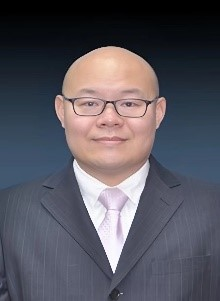
\includegraphics[width=1in,height=1.25in,clip,keepaspectratio]{xiaobo.png}}]{Xiaobo Qu} is a chair professor at the School of Vehicle and Mobility, Tsinghua University, China. He is also an elected Member of Academia Europaea, the Academy of Europe, since August 2020, and a Fellow of the Institution of Engineering and Technology (IET). His research is focused on enhancing urban mobility systems by incorporating emerging technologies, particularly for emergency
services and connected automated vehicles. He has authored or co-authored over 120 journal articles published in top-tier journals, including 14 ESI highly cited papers. He serves as an editor for 10 journals, including the Editor in Chief of Communications in Transportation Research, and Executive Editor in Chief of Journal of Intelligent and Connected Vehicles. To date, Dr. Qu has secured research funding well above 10 million Euros from the Australian Research Council, Swedish Innovation Agency Vinnova, STINT, and the European Union. He has been invited to serve as a panel/assessor for prestigious funding scheme such as the Australian Research Council Centre of Excellence (35 million AUD each), Future Fellowship (career grant, 1 million AUD each), Netherlands NWO VICI (career grant, 2.5 million Euros each), Hong Kong Research Council theme based scheme (30 million HKD each), Singapore Ministry of Education Thematic Research Program (5 million SD each), and the European Research Council, etc.
\end{IEEEbiography}






\end{document}







